\subsection{Einleitung}
In der heutigen Zeit nimmt die Technik einen großen Einfluss auf unser Leben.
Jeder durchschnittliche Haushalt besitzt mindestens einen Computer mit
Internetanschluss und die meisten Leute haben heutzutage auch ein Smartphone.
Selten allerdings bleibt es bei diesen beiden Gerätschaften und so kommt zum Beispiel
ein Notebook für die Schule oder für den Arbeitsplatz zum Einsatz. Oftmals
müssen dabei die selben Dateien auf verschiedenen Geräten bearbeitet werden und
das möglichst ohne \glspl{versionconflict}. Daten müssen von jedem
Gerät und zu jederzeit erreichbar sein, weshalb Cloud- und
Dateisynchronisationsdienste einen immer größer werdenden Stellenwert bekommen.
Das Verwalten beziehungsweise die Verarbeitung von Daten in einer
zentrale Stelle, meistens einem Server und die dahinter liegende Datenbank des
jeweiligen Anbieters, soll dabei mit hoher Uptime den dauerhaften Zugriff auf
die eigenen Dateien sicherstellen.

\subsection{Funktionsweise üblicher Dateisynchronisationsdienste}
Die Idee hinter \sblit basiert auf den sicherheitsbezogenen Problemen, die mit
der Speicherung von Daten auf einer zentralen Stelle einhergehen. Die
Erleuterung der Funktionsweise üblicher Dateisynchronsationsdienste soll beim
Verstehen der grundsätzlichen Idee hinter \sblit helfen.

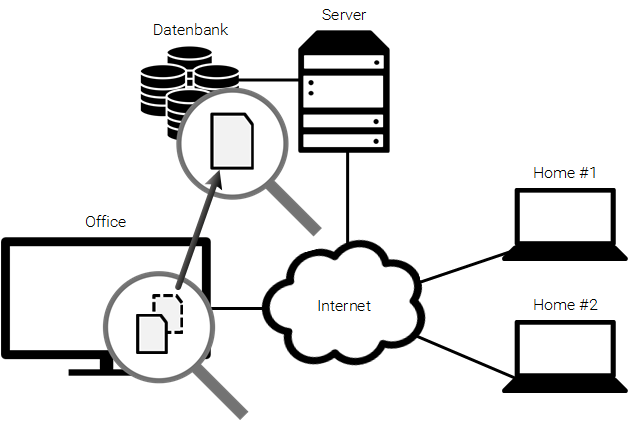
\includegraphics[]{images/Dropbox_1}
Üblich gehandhabtes Uploaden einer Datei.

Bei der Synchronisation einer Datei von einem Heimrechner zu einem Laptop am
Arbeitsplatz oder in der Schule wird eine Kopie dieser Datei auf den vom
Betreiber zur Verfügung gestellten Cloadspeicher beziehungsweise Server
hochgeladen und dort gespeichert. Der Sender behält dabei die Originaldatei.

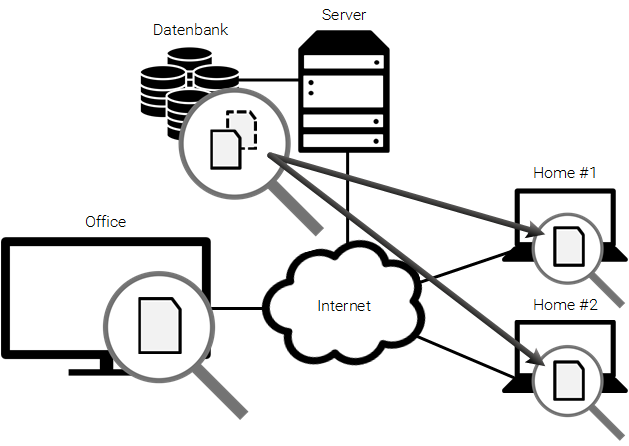
\includegraphics[]{images/Dropbox_2}
Üblich gehandhabtes Downloaden einer Datei.

Wenn der Laptop (TODO) in diesem Beispiel verfügbar ist, wird er über die Änderung
im Cloadspeicher informiert und lädt die Änderung, in diesem Fall die Datei von
dem Server herunter. Die Datei wurde somit über eine zentrale Stelle, hier den
Server synchronisiert.
